\documentclass[]{beamer}
%\documentclass[french,handout]{beamer}

\usepackage{tikz}
\usetikzlibrary{calc}
\usetikzlibrary{positioning}

\usepackage[T1]{fontenc}
\usepackage[utf8]{inputenc}
%\usepackage{mathptmx}
\usepackage[scaled=0.9]{helvet}
\usepackage{tcolorbox}

\usepackage[ruled,lined,longend]{algorithm2e}
\usepackage{tikz}
\usetikzlibrary[topaths]
\usetikzlibrary{arrows.meta,shapes.arrows}


%\usepackage{pgf}
%\usepackage{babel}
\usepackage{eurosym}
\usepackage{mathabx}

\graphicspath{{images/}}

\title[Julia]{Julia tutorial (3)\\ \textbf{MultiObjective Metaheuristic Implementation}}

\date{June 2024}
\author{Prof. Dr. Antonio J. Nebro$^1$ and Prof. Dr. Xavier Gandibleux$^2$}\bigskip
\institute{1: Universidad de Málaga, Spain\\ 2: Nantes Université, France} 
%}

\DeclareMathOperator{\conv}{\rm conv}
\DeclareMathOperator{\cl}{\rm cl}
\newcommand{\mR}{\mathbb{R}}
\newcommand{\mN}{\mathbb{N}}
\newcommand{\mZ}{\mathbb{Z}}
\newcommand{\mB}{\mathbb{B}}
\newcommand{\ab}{\par\noindent}

\definecolor{colorTD}{rgb}{0.0,0.6,0.7}
\definecolor{colorEL}{rgb}{0.7,0.6,0.0}
\definecolor{BLANC}{rgb}{1.0,1.0,1.0}
\definecolor{ROUGE}{rgb}{1.0,0.0,0.0}
\definecolor{BLEU}{rgb}{0.20,0.22,0.69}
\definecolor{GRIS}{rgb}{0.5,0.5,0.5}
\definecolor{nred}{rgb}{0.8,0.1,0.1}
\definecolor{ngreen}{rgb}{0,0.7,0.4}
\definecolor{nblue}{rgb}{0.2,0.5,0.8}
\definecolor{npink}{rgb}{0.25,0.04,0.87}
\newcommand*{\red}[1]{{\color{nred}#1}}
\newcommand*{\green}[1]{{\color{ngreen}#1}}
\newcommand*{\blue}[1]{\textcolor{nblue}{#1}}
\newcommand*{\pink}[1]{{\color{npink}#1}}
%\colorlet{BLEU}{Blue}
\newcommand{\grisc}[1]{\color{black!20}#1}

\setbeamertemplate{navigation symbols}{} 
\setbeamertemplate{footline}
{ 
\makebox[0.45\textwidth][l] {\hspace{2em} Metaheuristics International Conference 2024}  \hfill 
\includegraphics[height=0.6cm]{logo3ptsJulia.png} \hfill
\makebox[0.45\textwidth][r]{\href{mailto:Xavier Gandibleux@Univ-Nantes.fr}{Xavier Gandibleux@Univ-Nantes.fr} \quad\quad\insertframenumber\hspace{1em}}
\vskip5pt%
}
\setbeamercovered{transparent}

\begin{document}

% 
% ======================================================================================
%

\begin{frame}
  \titlepage
  \vspace{-1cm}
\end{frame}


\setbeamertemplate{footline}
{ 
\makebox[0.45\textwidth][l] {\hspace{2em} Metaheuristics with Julia}  \hfill 
\includegraphics[height=0.4cm]{logo3ptsJulia.png} \hfill
\makebox[0.45\textwidth][r]{\href{mailto:Xavier Gandibleux@Univ-Nantes.fr}{Xavier Gandibleux@Univ-Nantes.fr} \quad\quad\insertframenumber\hspace{1em}}
\vskip4pt%
}


% 
% -------------------------------------------------------------------------------------------------------------------------------------------------------
%
\begin{frame}[fragile]
  \frametitle{Multiobjective Optimization Problem (MOP)}

\[
\begin{array}{clrclrrrl}
\min   & F(x)   \\
s.t.     & x  \ \in \ X
\end{array}
\]


\vspace{-2mm}
\noindent 
where:
\vspace{2mm}
%\vfill
$$
\begin{array}{rcl}
%
X \subseteq\mR^n  & \longrightarrow & \hbox{the set of feasible solutions}\\
Y=F(X)\subseteq \mR^{\red{p}} & \longrightarrow & \hbox{the set of images}\\
\notag
\end{array}
$$
\pause

\hspace{0mm}Computing sets $Y_N$ and $X_E$ for MOP:

\vspace{0mm}

\begin{center}
{$y=F(x)$\medskip\\
$y^*\in Y$ is \textcolor{purple}{nondominated}, if $\not\exists\, y\in Y$ such that $y_i\leq y^*_i,~\forall i$ and $ y\not= y^*$.\\
			$\textcolor{purple}{Y_N}$ is the set of nondominated points.\medskip\\
			$x^*\in X$ is \textcolor{purple}{efficient} if $y^*$ is nondominated.\\
			$\textcolor{purple}{X_E}$ is a complete set of efficient solutions.}

\end{center}
\vspace{5mm}


\end{frame}

% 
% -------------------------------------------------------------------------------------------------------------------------------------------------------
%

\begin{frame}
  \frametitle{Example 1}
\vspace{3mm}

\textbf{Compute $X_E$ and $Y_N$ for the following 2-IP}:
\vspace{2mm}

    \[
\begin{array}{crrcrrrl}
\max z_1 & = & x_1 & + & x_2  \\
\min z_2 & = & x_1 & + & 3x_2 \vspace{2mm}\\
s.t. & & 2x_1 & + &  3x_2 & \le & 30 \\
    &&  3x_1 & + &  2x_2 & \le & 30 \\
    &&   x_1 & - &   x_2 & \le & 5.5 \vspace{2mm}\\
    &&   x_1 & , &   x_2 & \in & \mathbb{N}
\end{array}
\]
\vspace{0mm}

\vfill

\end{frame}

% ================================================================
% ================================================================
% ================================================================

\begin{frame}

\centerline 
{\Large \textbf{1. \ Exact resolution}}

\end{frame}

% 
% -------------------------------------------------------------------------------------------------------------------------------------------------------
%

\begin{frame}
  \frametitle{Exact resolution}
\vspace{3mm}

%\begin{itemize}
%\item \textbf{Compute $X_E$ and $Y_N$ for the following 2-IP}:
%\vspace{-1mm}
%
%    \[
%\begin{array}{crrcrrrl}
%\max z_1 & = & x_1 & + & x_2  \\
%\min z_2 & = & x_1 & + & 3x_2 \vspace{2mm}\\
%s.t. & & 2x_1 & + &  3x_2 & \le & 30 \\
%    &&  3x_1 & + &  2x_2 & \le & 30 \\
%    &&   x_1 & - &   x_2 & \le & 5.5 \vspace{2mm}\\
%    &&   x_1 & , &   x_2 & \in & \mathbb{N}
%\end{array}
%\]
%\vspace{0mm}
%
%\item 
\textbf{Easy in Julia with these packages:}
\vspace{3mm}
\begin{itemize}
\item Model: \\ \texttt{JuMP}\vspace{1.5mm}
\item Algorithm: \\ \texttt{MultiObjectiveAlgorithms}\vspace{1.5mm}
\item Solver: \\ \texttt{HiGHS}, \texttt{Gurobi}, etc.
\end{itemize}

%\end{itemize}


\end{frame}

% 
% -------------------------------------------------------------------------------------------------------------------------------------------------------
%

\begin{frame}
  \frametitle{From \ {\large \texttt{vOptGeneric.jl}} \ to \ {\large \texttt{MultiObjectiveAlgorithms.jl}}}
\vspace{3mm}

vOptSolver (vOptGeneric and vOptSpecific)\vspace{-2mm}\\
    \smallskip
    {\small
    \url{https://github.com/vOptSolver}    
    }
% \bigskip
    \smallskip

 {\scriptsize
\begin{itemize}
    \item[] 2015: Kick-off of vOpt ANR/DFG project\vspace{-1.25mm}\\
    \item[] 2017: Introduction of vOptSolver (vOptGeneric, vOptSpecific)\vspace{1.25mm}\\
    \begin{columns}
      \begin{column}{0.05\textwidth}
      \end{column}
      \begin{column}{0.85\textwidth}
              {\tiny
Xavier Gandibleux, Gauthier Soleilhac, Anthony Przybylski, Stefan Ruzika. vOptSolver: an open source software environment for multiobjective mathematical optimization. \textit{IFORS2017: 21st Conference of the International Federation of Operational Research Societies}. July 17-21, 2017. Quebec City (Canada).\vspace{0.5mm}\\}
      \end{column}
      \end{columns}

    
    \item[] 2018: Julia 1.0\vspace{-1.25mm}\\
    \item[] 2019: End of vOpt project   \vspace{-1.25mm}\\
    \item[] 2019: First discussions on discourse/new design of MOO in JuMP\vspace{-1.25mm}\\
    \item[] 2022: JuMP 1.0\vspace{-1.25mm}\\
    \item[] 2023: Introduction of MultiObjectiveAlgorithms\vspace{-1.25mm}\\
    \item[] 2023: End of vOptGeneric
\end{itemize}
}
    \smallskip
    \pause
    
    
JuMP\vspace{-2mm}\\
    \smallskip
    {\small
    \url{https://jump.dev/}
    }\vspace{0.5mm}\\
    \begin{columns}
      \begin{column}{0.05\textwidth}
      \end{column}
      \begin{column}{0.85\textwidth}
              {\tiny Miles Lubin. The state of JuMP.
              \textit{JuliaCon 2023: The 10th Annual JuliaCon - Co-Located with JuMP-dev}, July 25th - 29th, 2023. MIT, Cambridge, (USA). \vspace{0mm}\\}
      \end{column}
      \end{columns}     
    \medskip

MultiObjectiveAlgorithms (MOA) \vspace{-2mm}   \\
    \smallskip
    {\small
    \url{https://github.com/jump-dev/MultiObjectiveAlgorithms.jl}
    }    \vspace{0.5mm}\\
    
    \begin{columns}
      \begin{column}{0.05\textwidth}
      \end{column}
      \begin{column}{0.85\textwidth}
              {\tiny Oscar Dowson, Xavier Gandibleux, Gokhan Kof. From vOptGeneric.jl to MultiObjectiveAlgorithms.jl \quad
              \textit{JuliaDays 2023}, 4-6 October 2023. Paris (France). \vspace{0mm}\\}
      \end{column}
      \end{columns}    
      

\end{frame}


% 
% -------------------------------------------------------------------------------------------------------------------------------------------------------
%

\begin{frame}
  \frametitle{Getting Started}
\vspace{3mm}

\hspace{-2mm}Install:
\vspace{1mm}
{\scriptsize
\begin{tcolorbox}[arc=1ex, colback=black!20, colframe=black!20, left=3pt, right=3pt, top=3pt, bottom=2pt]
\texttt{ \hspace{-1.5mm}\green{julia>}  using Pkg}
%$\mbox{}$\hspace{0mm}   Pkg.add("JuMP")}
\end{tcolorbox}  
\vspace{1mm}
\pause
\begin{tcolorbox}[arc=1ex, colback=black!20, colframe=black!20, left=3pt, right=3pt, top=3pt, bottom=2pt]
\texttt{ \hspace{-1.5mm}\green{julia>}  Pkg.add("JuMP")}
\end{tcolorbox}  
\vspace{1mm}
%\pause
\begin{tcolorbox}[arc=1ex, colback=black!20, colframe=black!20, left=3pt, right=3pt, top=3pt, bottom=2pt]
\texttt{ \hspace{-1.5mm}\green{julia>}   Pkg.add("MultiObjectiveAlgorithms")}
\end{tcolorbox}
\vspace{1mm}
\pause
\begin{tcolorbox}[arc=1ex, colback=black!20, colframe=black!20, left=3pt, right=3pt, top=3pt, bottom=2pt]
\texttt{ \hspace{-1.5mm}\green{julia>}   Pkg.add("HiGHS")}
\end{tcolorbox}
%\pause
\vspace{3mm}
}

%\hspace{-2mm}Setup:
%\vspace{1mm}
%\begin{tcolorbox}[arc=1ex, colback=blue!20, colframe=blue!20, left=3pt, right=3pt, top=3pt, bottom=2pt]
%\texttt{ \hspace{-2mm}  using JuMP}
%\end{tcolorbox}  
%\vspace{-1mm}
%\begin{tcolorbox}[arc=1ex, colback=blue!20, colframe=blue!20, left=3pt, right=3pt, top=3pt, bottom=2pt]
%\texttt{ \hspace{-2mm}  using HiGHS}
%\end{tcolorbox}  
%\vspace{1mm}

\end{frame}


% 
% -------------------------------------------------------------------------------------------------------------------------------------------------------
%

\begin{frame}
  \frametitle{Example 1 (Con't)}
\vspace{3mm}


%\hspace{-2mm}

      {\scriptsize
    \begin{columns}
      \begin{column}{0.5\textwidth}
    \[
\begin{array}{crrcrrrl}
\max z_1 & = & x_1 & + & x_2  \\
\min z_2 & = & x_1 & + & 3x_2 \vspace{2mm}\\
s.t. & & 2x_1 & + &  3x_2 & \le & 30 \\
    &&  3x_1 & + &  2x_2 & \le & 30 \\
    &&   x_1 & - &   x_2 & \le & 5.5 \vspace{2mm}\\
    &&   x_1 & , &   x_2 & \in & \mathbb{N}
\end{array}
\]

      \end{column}
      \begin{column}{0.5\textwidth}


\begin{tcolorbox}[arc=1ex, colback=black!20, colframe=black!20, left=3pt, right=3pt, top=3pt, bottom=2pt]
%\texttt{ \hspace{-2mm}\green{julia>}  using JuMP, HiGHS}\\
\texttt{ \hspace{-1.5mm}\green{julia>}  c1 = [1,1]}\\
\texttt{ \hspace{-2mm}\green{julia>}  c2 = [1,3]}\\
\texttt{ \hspace{-2mm}\green{julia>}  A  = [2 3; 3 2; 1 -1]} \\
\texttt{ \hspace{-2mm}\green{julia>}  b  = [30, 30, 5.5]}
\end{tcolorbox} 
      \end{column}
      \end{columns} 
}      

\vspace{3mm}


    \begin{columns}
      \begin{column}{0.5\textwidth}
      Decision space:
      
      \begin{center}
      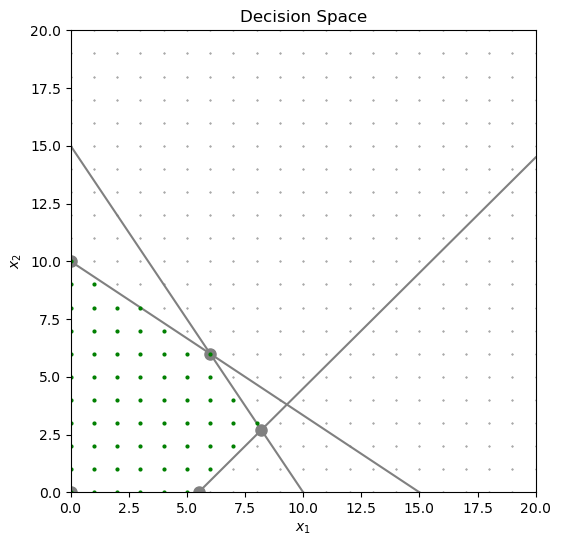
\includegraphics[height=4.25cm]{decisionSpace.png} 
       \end{center}
      \end{column}
      \begin{column}{0.5\textwidth}
      Objective space:
      
      \begin{center}
      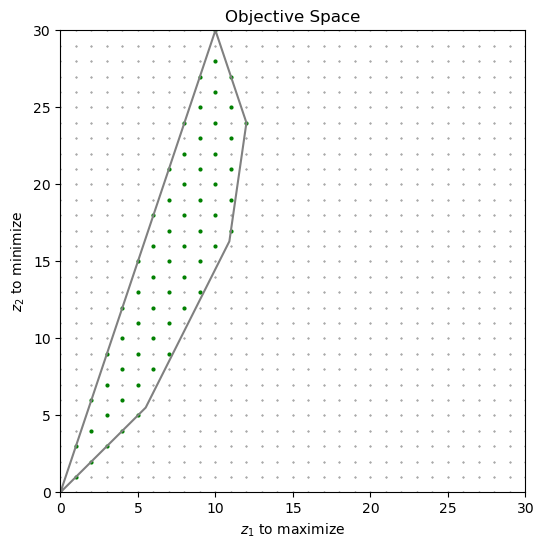
\includegraphics[height=4.25cm]{objectiveSpace.png} 
       \end{center}
      \end{column}
      \end{columns} 

\end{frame}



% 
% -------------------------------------------------------------------------------------------------------------------------------------------------------
%

\begin{frame}
  \frametitle{Example 1 (Con't)}
\vspace{3mm}


%\hspace{-2mm}
Write the corresponding  2-IP model with \texttt{JuMP}

{\scriptsize
\begin{tcolorbox}[arc=1ex, colback=black!20, colframe=black!20, left=3pt, right=3pt, top=3pt, bottom=2pt]
\texttt{ \hspace{-1.5mm}\green{julia>}  using JuMP, HiGHS}\\
\texttt{ \hspace{-2mm}\green{julia>}  import MultiObjectiveAlgorithms as MOA}
\end{tcolorbox} 


\begin{tcolorbox}[arc=1ex, colback=black!20, colframe=black!20, left=3pt, right=3pt, top=3pt, bottom=2pt]
\texttt{ \hspace{-1.5mm}\green{julia>} model = Model( ) }\\
\texttt{ \hspace{-2mm}\green{julia>} @variable(model, x1$\ge$0, Int)}\\
\texttt{ \hspace{-2mm}\green{julia>}  @variable(model, x2$\ge$0, Int)}\\
\texttt{ \hspace{-2mm}\green{julia>}  @expression(model, fct1, x1 + x2)     \hfill  \# to maximize}\\
\texttt{ \hspace{-2mm}\green{julia>}  @expression(model, fct2, x1 + 3 * x2)  \hfill \# to minimize}\\
\texttt{ \hspace{-2mm}\green{julia>}  @objective(model, Max, [fct1, (-1) * fct2]))}\\
\texttt{ \hspace{-2mm}\green{julia>}  @constraint(model, 2*x1 + 3*x2 $\le$ 30))}\\
\texttt{ \hspace{-2mm}\green{julia>}  @constraint(model, 3*x1 + 2*x2 $\le$ 30))}\\
\texttt{ \hspace{-2mm}\green{julia>}  @constraint(model,   x1 -   x2 $\le$ 5.5))}
%\texttt{ \hspace{-2mm}\green{julia>}  }
\end{tcolorbox} 

\begin{tcolorbox}[arc=1ex, colback=black!20, colframe=black!20, left=3pt, right=3pt, top=3pt, bottom=2pt]
\texttt{ \hspace{-1.5mm}\green{julia>}   print(model)}
\end{tcolorbox} 
}


\end{frame}

% 
% -------------------------------------------------------------------------------------------------------------------------------------------------------
%

\begin{frame}
  \frametitle{Example 1 (Con't)}
\vspace{3mm}


Setup the MIP solver, e.g. \texttt{HiGHS}

{\scriptsize
\begin{tcolorbox}[arc=1ex, colback=black!20, colframe=black!20, left=3pt, right=3pt, top=3pt, bottom=2pt]
\texttt{ \hspace{-1.5mm}\green{julia>} set\_optimizer(model,()->MOA.Optimizer(HiGHS.Optimizer)) }
\end{tcolorbox} 
}
\bigskip

Setup the algorithm: $\epsilon$-constraint; step=1 (default value)

{\scriptsize
\begin{tcolorbox}[arc=1ex, colback=black!20, colframe=black!20, left=3pt, right=3pt, top=3pt, bottom=2pt]
\texttt{ \hspace{-1.5mm}\green{julia>} set\_attribute(model, MOA.Algorithm(), MOA.EpsilonConstraint()) }
\end{tcolorbox} 
}
\bigskip

Optimize the MOO problem

{\scriptsize
\begin{tcolorbox}[arc=1ex, colback=black!20, colframe=black!20, left=3pt, right=3pt, top=3pt, bottom=2pt]
\texttt{ \hspace{-1.5mm}\green{julia>}  optimize!(model) }
\end{tcolorbox} 
}

\end{frame}

% 
% -------------------------------------------------------------------------------------------------------------------------------------------------------
%

\begin{frame}
  \frametitle{Example 1 (Con't)}
\vspace{3mm}


Get $X_E$ and $Y_N$

{\scriptsize
\begin{tcolorbox}[arc=1ex, colback=black!20, colframe=black!20, left=3pt, right=3pt, top=3pt, bottom=2pt]
\texttt{ \hspace{-1.5mm}\green{julia>}  for i in 1:result\_count(model) }\\
\texttt{ \hspace{-2mm}\green{julia>}      \qquad z1\_opt = objective\_value(model; result = i)[1]}\\
\texttt{ \hspace{-2mm}\green{julia>}      \qquad z2\_opt = -1 * objective\_value(model; result = i)[2] }\\
\texttt{ \hspace{-2mm}\green{julia>}      \qquad x1\_opt = value(x1; result = i)}\\
\texttt{ \hspace{-2mm}\green{julia>}      \qquad x2\_opt = value(x2; result = i) }\\
\texttt{ \hspace{-2mm}\green{julia>}  end }
\end{tcolorbox} 
}

\vspace{0mm}


    \begin{columns}
      \begin{column}{0.5\textwidth}
      
      \begin{center}
      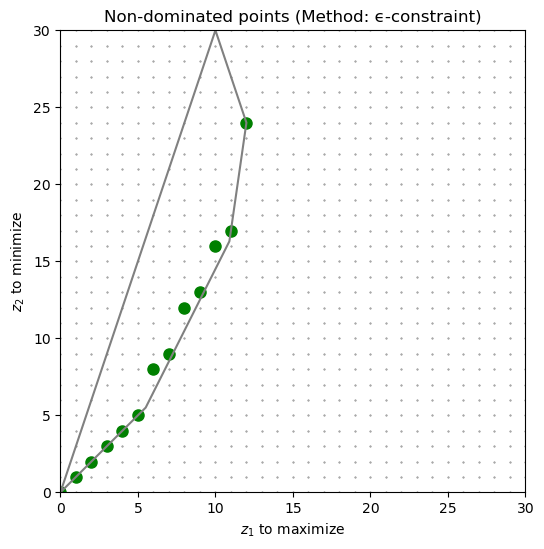
\includegraphics[height=4.25cm]{ndPoints.png} 
       \end{center}
      \end{column}
      \begin{column}{0.5\textwidth}
      
      \begin{center}
      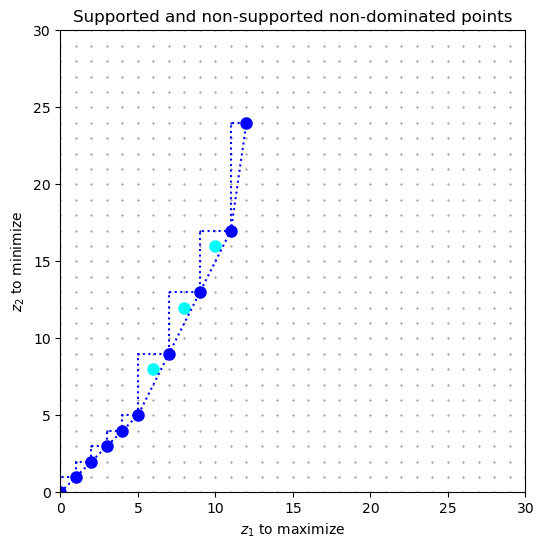
\includegraphics[height=4.25cm]{seNe.png} 
       \end{center}
      \end{column}
      \end{columns} 

\end{frame}

% ================================================================
% ================================================================
% ================================================================

\begin{frame}

\centerline 
{\Large \textbf{1. \ Heuristic resolution}}

\end{frame}

%
%-----------------------------------------------------------
%
\begin{frame}

You enter on the scene Antonio...
\bigskip

During your talk, could you illustrate the resolution of the example 1 with MetaJul?

\end{frame}

%
%-----------------------------------------------------------
%
\begin{frame}
  \frametitle{References}
\vspace{3mm}

{\scriptsize
\begin{itemize}

\item 
Jeff Bezanson, Alan Edelman, Stefan Karpinski and Viral B. Shah.
Julia: A Fresh Approach to Numerical Computing. 
\textit{SIAM Review}, 59: 65--98. 2017.
\vspace{2mm}

\item 
 Miles Lubin, Oscar Dowson, Joaquim {Dias Garcia}, Joey Huchette, Beno{\^i}t Legat, Juan Pablo Vielma.
{JuMP} 1.0: {R}ecent improvements to a modeling language for mathematical optimization.
\textit{Mathematical Programming Computation}.
2023.
\vspace{2mm}


\item JuMP\\
    \url{https://jump.dev/}
\vspace{2mm}

\item MultiObjectiveAlgorithms (MOA)    \\
    \url{https://github.com/jump-dev/MultiObjectiveAlgorithms.jl}
\vspace{2mm}
    
\end{itemize}
}
   
\end{frame}





\end{document}
% 
% -------------------------------------------------------------------------------------------------------------------------------------------------------
%

\begin{frame}
%  \frametitle{Slides suivants...}
  
      \vspace{7mm}
    \centerline{
\includegraphics[height=6cm]{imageMire.png}}
    \vspace{5mm}
    
%  \href{run:./FctOI-1-1-THEME1representations.pdf}{\centerline{\Large{\textcolor{nblue}{Next: Getting started}}}}
  
\end{frame}

  
\end{document}  



    


